\documentclass[a4paper, 12pt]{article}

\usepackage[utf8]{inputenc}
\usepackage[T1]{fontenc}
\usepackage[french]{babel}
\usepackage[top=2cm, bottom=2cm, left=1.5cm, right=1.5cm,headheight=16pt]{geometry}
\usepackage{lmodern}

\addto\captionsfrench{%
    \renewcommand{\tablename}{\textsc{Tableau}}%
}

\usepackage{cover-page}
\title{Finite State Transducers Just-In-Time Compiling}
\subtitle{Do you hear the bytecode ?}
\author{Émilien Boulben\\Victor Delepine\\Corentin Peuvrel}
\location{Paris}
\date{\today}
\blurb
{
    Institut Supérieur d'Électronique de Paris\\
    \textbf{Projet de Fin d'Études}\\
    ~\\
    Reponsable: M. Hugueney
}

\usepackage{fancy-perso}
\usepackage{lastpage}
\headerleft{Finite State Transducer Just-In-Time Compiling}
\headerright{Institut Superieur d'Électronique de Paris}
\footerleft{É.Boulben, V.Delepine, C.Peuvrel}
\footerright{\hyperlink{Contents}{Table des matières}}

\usepackage{parskip}
\setlength{\parindent}{18pt}

\usepackage{listings}
\usepackage{upquote}
\usepackage{graphicx}
\usepackage{listings}
\usepackage{xcolor}

\makeatletter
\newcommand{\lstdefinestylecustom}[3] {%
    \ifnum\pdfstrcmp{#3}{x86masm}=0
    \lstdefinestyle{#1}{
        numbers=left,
        stepnumber=1,
        numberstyle=\scriptsize,
        belowcaptionskip=1\baselineskip,
        captionpos=b,
        breaklines=true,
        frame=L,
        xleftmargin=\parindent,
        language=[#3]#2,
        showstringspaces=false,
        basicstyle=\footnotesize\ttfamily,
        keywordstyle=\bfseries\color{green!40!black},
        commentstyle=\itshape\color{purple!40!black},
        identifierstyle=\color{blue},
        stringstyle=\color{orange},
        comment=[l]\#,
    }
    \else
    \lstdefinestyle{#1}{
        numbers=left,
        stepnumber=1,
        numberstyle=\scriptsize,
        belowcaptionskip=1\baselineskip,
        captionpos=b,
        breaklines=true,
        frame=L,
        xleftmargin=\parindent,
        language=#2,
        showstringspaces=false,
        basicstyle=\footnotesize\ttfamily,
        keywordstyle=\bfseries\color{green!40!black},
        commentstyle=\itshape\color{purple!40!black},
        identifierstyle=\color{blue},
        stringstyle=\color{orange},
    }
    \fi
}
\makeatother

\lstdefinestylecustom{custombash}{bash}{}
\lstdefinestylecustom{customc}{C}{}
\lstdefinestylecustom{customasm}{Assembler}{x86masm}

\usepackage[pdftex,breaklinks,linktocpage,unicode]{hyperref}
\hypersetup{
    unicode=false,          % non-Latin characters in Acrobat’s bookmarks
    pdftoolbar=true,        % show Acrobat’s toolbar?
    pdfmenubar=true,        % show Acrobat’s menu?
    pdffitwindow=false,     % window fit to page when opened
    pdfstartview={FitH},    % fits the width of the page to the window
    pdftitle={Finite State Transducer Just-In-Time Compiling},    % title
    pdfauthor={Émilien Boulben, Victor Delépine, Corentin Peuvrel},     % author
    pdfsubject={FST, bytecode, optimisation},   % subject of the document
    pdfcreator={Émilien Boulben},   % creator of the document
    pdfproducer={Émilien Boulben}, % producer of the document
    pdfkeywords={FST, assembler, bytecode, just, time, java}, % list of keywords
    pdfnewwindow=true,      % links in new window
    colorlinks=true,       % false: boxed links; true: colored links
    linkcolor=black,          % color of internal links (change box
    % color with linkbordercolor)
    linktoc=all,
    citecolor=green,        % color of links to bibliography
    filecolor=magenta,      % color of file links
    urlcolor=cyan           % color of external links
}


\usepackage{amsmath}

\begin{document}

\maketitle

\newpage
\clearpage
\pagenumbering{Roman}
\setcounter{page}{1}
\footercenter{\textbf{\thepage}}
\fancyperso{HL}{HR}{FL}{FC}{}

\hypertarget{Contents}{}
\tableofcontents
\newpage
\lstlistoflistings
\newpage
\listoftables
\newpage
\listoffigures

\newpage
\clearpage
\pagenumbering{arabic}
\setcounter{page}{1}
\footercenter{\textbf{Page \thepage/\pageref{LastPage}}}
\fancyperso{HL}{HR}{FL}{FC}{FR}

\section*{Introduction}
\addcontentsline{toc}{section}{\protect\numberline{}Introduction}

Les FST -- Finite State Transducers ou en français Transducteur fini -- sont des automates
finis particuliers puique possédant une sortie. Ils sont enormément utilisés par les
moteurs de recherche puisqu'ils permettent d'associer à un mot une valeur numérique
unique. C'est l'indexation.


Nous savons donc déjà transformer le texte en valeur exploitable ensuite
(par comparaison avec un disctionnaire par exemple).
Mais de part les quantités non négligeable de texte à analyser, et ce le plus rapidement
possible, il est essentiel de continuer les recherches afin de réussir à optimiser
cette transformation.


Seulement en ingénérie l'optimisation n'est pas tout, il faut aussi pouvoir simplement déployer les
solutions sur différents serveurs : une solution trop complexe même performante sera très
coûteuse à long termes et donc probablement pas choisie.
C'est alors qu'intervient ce projet.


Il s'agit de faire une étude sur la faisabilité et la pertinence d'une nouvelle manière
d'indexer le texte en java, L'objectif n'est pas de faire mieux que la référence qu'est Lucène,
mais de déterminer s'il est possible de faire mieux en utilisant cette méthode.\newline


Nous allons avec ce projet chercher à déterminer si un interpréteur de FST reposant sur la
compilation à la volée est viable en java.

\newpage
\section{Analyse préalable}

\subsection{Le projet en détail}

Pour pallier à des problèmes de performance et de distribution de la solution lors de
l'indexation d'un texte en suivant une FST il est important de penser à de nouvelles
solutions qui pourront éventuellement challenger la librairie de référence sur ce sujet :
Lucène. L'objectif n'est pas d'y parvenir, mais de déterminer si cela est possible avec
une solution qui a été imaginée par M. Hugueney et M. Marty.


Dans Lucène lors de la création d'une FST une structure de données est stockée en ram et
le texte la parcourt pour connaître le résultat. Afin de gagner en performance en termes
de temps d'exécution lors de cette étape, ne serait-il pas mieux de pouvoir avoir un code
simple mais conséquent en taille qui soit parfaitement adapté à la FST désirée ? Finalement,
plutôt que créer une structure générique, générer un code dédié à la FST en étude et l'optimiser
au mieux en bafouant tous les principes de développement afin de gagner en temps d'exécution.
La lisibilité est sacrifiée mais ce n'est pas très important compte tenu que ce code n'a pas
destination à être lu, seulement compilé puis parcouru.\newline


L'objectif du projet est de réussir à créer un programme Java qui génèrerait le code correspondant
à une FST donnée pour pouvoir parser du texte efficacement, d'abord en Java puis en bytecode.
Ensuite, faire une étude des performances et si possible les comparer avec les outils déjà existant.
Il est très important de documenter les difficultés rencontrées puisque l'objectif reste de
pouvoir se prononcer sur la faisabilité ou l'utilité d'un tel produit.

\subsection{Premières études}

Il nous a été très compliqué de comprendre ce qu'était une FST. Nous avons beaucoup investi de
temps à combler ce manque avec des résultats très mitigés. Il était très difficile avec toute la
documentation disponible de savoir par quoi commencer, surtout que souvent pour comprendre
certains concepts il nous fallut assimiler ce que les explications considéraient acquit.

Cette incompréhension du sujet fût à l'origine de bien des découragements, et il n'a pas toujours
été facile de nous remotiver les uns et les autres. Finalement c'est la pratique qui nous a apporté
le plus de réponse.\newline

Une FST qui permette l'indexation de texte, qu'est-ce ? Une simple structure de donnée. Un tableau
(voir \autoref{tab:fst1} et \autoref{tab:fst2}) ou un graphe (voir \autoref{fig:fst-dico1} et \autoref{fig:fst-dico2} peut la représenter).
Elle est construite par un algorithme à partir d'un dictionnaire qui associe à des mots des valeurs.
Enfin cela permet de parser du texte lettre à lettre (voir mots à mots) rapidement et en parallèle.


Une fois cette base essentielle partiellement comprise nous avons pris le courage de nous lancer
dans le code.

\subsection{Commencer quelque part}

Commencer à coder paraît simple et pourtant nous y avons rencontré de trop nombreuses difficultés.
Nous nous sommes heurtés à des nombreuses reprises à notre méconnaissances des FST, et n'arrivions
pas à dégager un cas simple sur lequel travailler et monter en compétence.

Nous avons aussi perdu du temps à partir sur du code inutile à ce moment du développement :
algorithmes de création d'une FST, tests en bytecode... Alors que ce n'était pas la priorité
à ce moment.\newline


C'est après une pause dans le projet que nous avons pu le reprendre d'un regard nouveau et
l'aborder avec un outil que nous maitrisons mieux pour générer du texte : bash. Par un découragement
général nous avons presqu'involontairement trouvé ce dont nous avions besoin pour nous lancer
avec efficacité dans le projet : un appui solide mais rapide à construire.

\newpage
\section{Les premiers essais}

\subsection{Générer du C en bash}

L'objectif ici n'était pas de réussir à faire quelque chose de fonctionnel, mais de comprendre
ce qu'il nous fallait faire. Pour ce faire nous avons finalement décidé de le faire avec les
langages que nous maitrisions le plus et que nous jugions les plus adaptés pour la situation : le
bash et le C.

\subsubsection{Le jeu de données}

Nous avons créé manuellement des FST très basique, reliées à un dictionnaire, afin de disposer
d'un jeu de test. Ils se trouvent en \autoref{sec:annexe:shell}.

Nous avons légèrement adapter le format défini par AT\&T pour décrire des FST dans un fichier texte.
Ce jeu de données servira pendant tout le projet en étant réadapté en Java par la suite.

\subsubsection{Fonctionnement}

Dans ce premier test nous prenons en entrée du script le fichier texte décrivant la FST,
puis générons un code C qui permette de parcourir cette FST.
Dans ce nouveau code point d'alorithme complexe : simplicité et naïvité sont ici ce que nous cherchons.
Nous espérons alors que la pratique nous permettra
de mieux comprendre le sujet.
De plus nous faisons confiance à gcc pour optimiser le code à la compilation.


La première étape pour construire ce script est bien sûr de prévoir la forme qu'aura le code C généré :
nous avons donc concentré nos premiers efforts à la généation d'une fonction contenant de multiples labels
correspondant chacun à un état (ou n\oe ud) et un switch qui, suivant la lettre courrante
se déplace à la lettre suivante grâce à un goto qui pointe sur le label du state/node suivant.
Nous returnons un code d'erreur si le token d'entrée n'est pas compatible avec la FST (le mot n'est pas
pris en compte par celle-ci et n'a pas de code associé).



Cette fonction prend comme seul paramètre d'entrée une chaine (tableau de char) --
qui sera le token d'entrée dont on veut connaitre la valeur -- et retourne le poids cumulé de
tous les arcs traversés, ou -1 en cas d'erreur.
Il faut remarquer qu'avec cette méthode on ne peut pas supporter de poids négatifs,
au risque d'avoir une collision entre le code d'erreur et un poids cumulé effectivement négatif.
Pour gérer ce cas, le plus simple serait d'utiliser errno.

Le code a été un peu moins simple que prévu pour pouvoir générer du C valide, en effet, il y a un
certain nombre de cas particuliers à prendre en compte afin de gérer correctement les erreurs ou
de multiples états de fins.



Au final, un état générera un code semblable à celui présent dans le \autoref{lst:node:example}
(pour un état appellé "7", qui possède
un arc pour le caractère 'X' avec un poids de 6 et qui va au node "21", et un arc pour
le caractère 'Y' avec un poids nulle et allant au node "42").
\begin{figure}
    \lstinputlisting[style=customc, caption=Un example de code généré pour un état,label=lst:node:example]{code/node1}
\end{figure}

On remarque la présence d'un compteur "pos" incrémenté de manière inconditionnel, vu que l'on se
déplace toujours un caractère par un caractère.

Pour pouvoir facilement lancer le programme généré, nous avons rajouté une fonction main qui appelle
juste notre fonction compute\_fst sur le premier argument de la command line,
rendant ainsi le programme autonome.

Il nous suffit donc, pour générer quelque chose d'utilisable de faire ceci :

\begin{align*}
    ./gen.sh\ file.fst\ |\ gcc\ -x\ c\ -o\ fst\ -
\end{align*}

Puis :

\begin{align*}
./fst\ LE\_TOKEN
\end{align*}

Les options sur gcc (on peut aussi rajouter un -O3 pour optimiser au maximum la compilation)
servant seulement de prendre l'entrée standard comme "fichier" source, puisque gen.sh affiche
le code généré sur la sortie standard.\newline


Les différents codes se situent en \autoref{sec:annexe:shell:c}, et plus précisément :
\begin{itemize}
    \item code bash : \autoref{lst:bashgen}
    \item Premier example de code C obtenu : \autoref{lst:cfst1}
    \item Second example de code C obtenu : \autoref{lst:cfst2}
\end{itemize}

\subsubsection{Les avantages}

Si le résultat n'avait que peu d'importance ici, ce début à une importance capitale dans ce projet
puisque c'est ce petit code qui nous a permis de mieux comprendre ce qui était attendu de nous,
comment le faire, et comment utiliser une FST.

\subsection{Générer de l'asmX86 en bash}

Sachant qu'on devrait sûrement au final généré du bytecode, nous avons décidé que, quitte à avoir du C,
autant aller jusqu'à générer directement de l'assembleur.
Pas spécialement pour être plus performant que le C (en effet, l'assembleur  généré par gcc
sera toujours plus efficace que celui que l'on peut faire à la main), mais pour avoir des idées
des problèmes que nous rencontrerons en bytecode.

Quand nous parlons d'assembleur, nous entendons "assembleur x86\_64" bien sûr,
soit l'assembleur qui est généré par gcc sur nos machines.


En donnant l'option "-S" à gcc, on obtient non pas un binaire éxécutable
mais un fichier ".s" qui contient le code assembleur généré (avant l'assemblage effectif en binaire).
En le générant pour nos sources C, nous avons pu faire du rétro-engineering dessus
et comprendre la marche à suivre pour notre deuxième script.

La première partie, pour adapter toutes les parties générées de manière statique, a été relativement aisée.
Par exemple, la déclaration de la fonction main, bien que plus longue et moins lisible qu'en C pouvait
être plus ou moins copié/collé par rapport à ce que générait gcc, et même si quelques lignes restaient
un peu mystérieuses au moment de la mise en place de "l'environnement" de la fonction, ce n'était
absolument pas bloquant.

À l'opposé, lorsqu'il a fallu adapter les parties générées dynamiquement, ce fut beaucoup moins simple.
Nous avons du, l'espace d'un instant, changer notre façon de programmer. En effet, l'assembleur
est tellement bas niveau que l'on ne dispose pas de toutes les "syntactic sugar" dont on a
tant l'habitude, nottamment pour le contrôle de flux. Par exemple, ce n'est pas si simple que
ce à quoi nous pourrions nous attendre de faire un "if (...) single\_instruction ;".
Il faut gérer deux sauts, les labels associés, potentiellement préparer un ou deux registres, etc...


Ce fût très amusant à faire, et moins complexe qu'imaginé grâce à l'exhaustivité de la documentation.
Néanmoins le temps passé dessus ne s'est révélé être aussi utile qu'escompté car nous le découvrirons
plus tard les problèmes rencontrés pour le bytecode sont d'un ordre totalement différents.\newline


Les différents codes se situent en annexe,annexe \autoref{sec:annexe:shell:asm}, et plus précisément :
\begin{itemize}
    \item code bash : \autoref{lst:bashgenasm}
    \item Premier example de code C obtenu : \autoref{lst:asmfst1}
    \item Second example de code C obtenu : \autoref{lst:asmfst2}
\end{itemize}

\newpage
\subsection{Adapter le travail précédent en Java}

Ici le travail fait précédemment avec la génération d'un fichier C s'est montré être très
utile. En effet cette étape a été traversée en quelques heures sans difficulté particulière.


Il nous suffit de séparer en trois cas l'étude d'un n\oe ud et de créer une méthode
particulière pour gérer intelligemment chaque cas. Le code est ajouté progressivement
dans un StringBuffer avant d'être retourné (pour être imprimé en console ou
dans un fichier).

Néanmoins cette étape ne fût absolument pas inutile puisqu'elle permit avec un cas simple
de s'essayer à la génération d'une classe en Java. Seulement elle ne convenait pas tout
à fait puisque nous avions recréé une manière de recréer des états et ce n'est pas
ce que nous voulions.

Finalement nous avions obtenu le code présent en annexe dans le \autoref{lst:javagen1}.

\subsection{Générer une structure de switch imbriqués en Java}

Le code précédent nous permit de prendre confiance à propos de le génération de code en Java.
Mais il s'agissait à présent de générer une structure en switch afin de s'approcher du
sujet.


Cette fois nous avons rencontré de nombreuses difficultés à cause d'une problématique
qui allait nous poursuivre pendant tout le projet : les switch ne sont pas voisins mais
imbriqués les uns dans les autres.
Ceci complexifia le problème mais nous avions finalement réussi grâce à un peu d'astuce
et des souvenirs de nos cours de programmation en A1 à écrire une méthode récursive
qui remplissait le StringBuffer au fur et à mesure et fermait en remontant dans la
stack les blocs ouverts.

Il nous fallu aussi prendre en compte le cas supplémentaire suivant : un état final n'étant
pas au bout de l'arbre de la FST (exemple : pour 'arbre' et 'arbres' le parcours du dit
arbre est le même excepté que pour 'arbre' l'état final est sur le e). Nous n'y avions pas
pensé auparavant et ce fut sources de bugs difficiles à identifier jusqu'à ce que
nous comprenions notre erreur.\newline


Le code final utilisé pour la génération se trouve dans le \autoref{lst:javagen2}.

\newpage
\section{Générer une FST}

\subsection{Le besoin}

Avant de compiler nos FST, il nous faut bien sûr les construire à partir de données
d'entrée et de données de sortie. Seulement pour faire des tests d'envergure nous
ne pouvions plus les construire à la main. Il nous fallait les construire automatiquement.

Pour ce faire, nous avons décidé d'utiliser un algorithme de construction directe de "Minimal acyclic subsequential transducers". Il s'agit de l'algorithme utilisé dans le projet Apache Lucene, pour la construction de leurs FST. Il permet de construire des transducteurs minimums pour des entrées et sorties données. Nous pouvons donc avoir des données de la forme :

\begin{table}[h]
    \centering
    \begin{tabular}{|l|l|}
        \hline
        In & Out \\
        \hline
        John & 1 \\
        Moth & 2 \\
        Mob & 3 \\
        \hline
    \end{tabular}
    \caption{Exemple de dictionaire}
    \label{tab:exemple1}
\end{table}

Note : Les mots en entrées doivent être triés dans l'ordre lexicographique pour
que l'algorithme fonctionne.

Cet algorithme nous permet d'être certain que le FST construit associera de manière unique la sortie 1 au mot John, la sortie 2 au mot Moth et la sortie 3 au mot Mob. Et ce même pour des millions d'entrées de cette forme.

De plus, étant utilisé par Lucene, cela nous permettra d'avoir une équivalence entre les FST que nous construisons et ceux construits par Lucene, afin qu'il soit possible de comparer les performances de notre méthode et celle de Lucene.

\subsection{Fonctionnement de l'algorithme}

L'algorithme est issu d'un papier de recherche qui date de 2001, écrit par Denis Maurel et Stoyan Mihov.
Il fonctionne pour tout type de données d'entrée/sortie, mais nous l'avons adapté en fixant pour sorties sont des nombres entiers par souci de simplicité (et nous le supposons de performance mais n'en avons pas de preuve).
L'algorithme parcourt les mots en entrée un par un, et cherche un préfixe commun entre le mot actuel et le mot du tour de boucle précédent. En déterminant ce préfixe commun, il est ensuite possible de réutiliser des états qui auraient déjà été créés lors du traitement d'un mot précédent (un peu comme dans un jeu de Scrabble). Petit à petit, on arrive donc à construire un Trie correct et à s'assurer que la valeur de sortie de chaque chaîne est unique.


\href{http://citeseerx.ist.psu.edu/viewdoc/summary?doi=10.1.1.24.3698}{Direct Construction of Minimal Acyclic Subsequential Transducers (2001)}

\subsection{Difficultés}

Il nous a été très difficile de comprendre le pseudo code et de l'implémenter correctement.
Nous avons du lors des premiers essais traverser de très nombreuses erreurs qui
ne nous permettaient pas d'avancer suffisemment. Finalement nous n'avons pas eu d'autre
choix que de l'implémenter en tout trois fois, en essayant à chaque fois d'avoir plus
de recul. Nous avons vraiment travaillé tous les trois ensemble sur le compréhension
(et non l'implémentation) par nécessité afin de pouvoir profiter des interprétations
de tous pour pouvoir avancer.


Aujourd'hui malgré tous nos efforts l'algorithme n'est pas entièrement fonctionnel :
\begin{itemize}
    \item Les états ne sont pas restitutés dans le bon ordre (bug mineur)
    \item Les poids ne sont pas correctement distribués sur tous les arcs, particulièrement lorsque les états finaux ne sont pas en bout de branche (bug majeur).
\end{itemize}

Nous n'avons pas réussi à déterminer l'origine de ces bugs.

\subsection{Résultat}

Pour le dictionnaire suivant :

\begin{table}[h]
    \centering
    \begin{tabular}{|l|l|}
        \hline
        In & Out \\
        \hline
        A      &  1 \\
        Aani   &  2 \\
        Aaron  &  3 \\
        Aaronic&  4 \\
        Aaronical      &  5 \\
        Aaronite       &  6 \\
        Aaronitic      &  7 \\
        Aaru   &  8 \\
        Ab     &  9 \\
Ababdeh & 10 \\
        \hline
    \end{tabular}
    \caption{Dictionaire utilisé pour tester l'algorithme}
    \label{tab:exemple2}
\end{table}

\begin{figure}[ht]
    \centering
    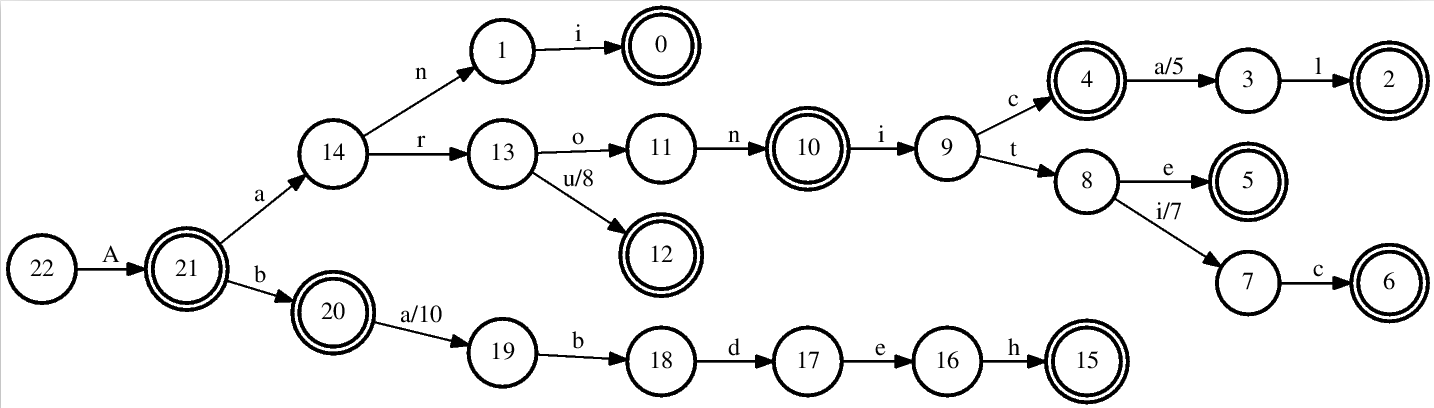
\includegraphics[scale=0.35]{algofst.png}
    \caption{La FST associée avec le \autoref{tab:exemple2} générée par l'algorithme}
    \label{fig:algo:fstgen}
\end{figure}

\newpage
\clearpage
\section{Idées d'amélioration et difficultés insurmontables}

Nous disposions à présent d'un algorithme perfectible mais utilisable qui permettait
de créer de grands FST. Nous avions aussi un moyen de générer du code Java pour
parcourir la FST donnée en argument. Le gros du travail commençait : utiliser ces outils
pour tester dans des conditions plus proches de celles réelles.

\subsection{Idées originelles}

\subsubsection{L'encodage}

Nous pensions au début du projet qu'il serait malin de changer l'encodage des caractères afin
de contourner les mauvaises performances liées à l'UTF16. Seulement pour des besoins
d'implémentation algorithmique nous avons très tôt pris la décision de travailler avec des
entiers plutôt que les charactères unicodes. Cela nécessite une transformation de l'entrée
avant de l'utiliser, mais cela aurait été nécessaire de toute manière.


Nous supposons en ayant fait ce choix avoir gagné en optimisation. Seulement il est
regrettable que nous n'ayons pas réussi à implémenter l'alogorithme avec des charactères
ou des string, car cela nous aurait permit de faire un véritable comparatif.

\subsubsection{Le traitement d'un texte en multithreading}

Nous avons très vite pensé à la manière par laquelle nous pourrions utiliser notre classe
générée avec une grande quantité de texte en entrée.
Nous avions comme idée de parcourir l'entrée afin d'y dinstinguer les mots (séparés par des
espaces) et de lancer le parcourt de la FST sur différentes mots en même temps, dans différents thread.
En effet, en divisant l'entrée et en prenant en compte les performances du Java en
multi-threading il est imaginable que les performances soient améliorées.
Hélas nous n'avons pas arrivé à cette étape à cause des difficultés à venir.

\subsection{Les difficultés les plus grandes}

\subsubsection{Compilation à la volée}

Afin d'automatiser le process de génération puis utilisation de classe, il est nécessaire
de la compiler. Seulement cela n'est pas simple en Java.
Nous avons essayé d'utiliser une des librairies fournies par Google pour le faire
mais nous n'avons pas réussi à la faire fonctionner correctement.

De plus, même compilée il nous fallait ensuite utiliser la reflexivité pour utiliser la
classe. Si bien que nous avions décidé de nous diriger vers le bytecode le plus vite possible
afin de contourner ce problème de compilation.

\subsubsection{Méthodes Java et la limitation 64Ko}

Lorsque nous commencions à tester le code généré avec des entrées beaucoup plus grandes
(un vrai dictionnaire avec quelques dizaines de millions d'entrée) notre première
surprise fût la taille de la classe générée : 129Mo. Plutôt gros pour du fichier texte.
Avant même d'aller plus loin nous étions très déçus de cette découverte sachant que dans le
projet Lucène 8 millions de mots occupaient 90Mo.


Mais notre plus mauvaise surprise eu lieu lors de la compilation. Nous nous attendions
à ce qu'il y ait une limite de la taile d'une classe ou méthode en Java et appréhendions
le résultat de cette compilation. Mais lorsque le compilateur nous dit explicitement
qu'une méthode ne pouvait pas dépasser 64Ko (ce que sera confirmé plus tard par de la lecture de documentions diverses) l'information était difficile à croire pour nous.
Une grande désillusion. Et pourtant nous n'étions pas au bout de nos peines.


En effet, de par la très grande variété de caractères présents dans les textes aujourd'hui
nous pouvions nous attendre à nous approcher de cette limite dès le premier switch, voir la
dépasser avant même d'avoir écrit la première imbrication!


Nous avons décidé de continuer malgré cette problématique qui semblait sans solution viable
dans tous les cas de figure afin de pouvoir étudier d'autres aspects du projet. Nous avons
donc changé la génération afin qu'une méthode soit créée à chaque 'case' d'un switch.
L'objectif est évident : réduire la taille des méthodes. Cette méthode utilisée est inspirée
de celle du "trampolining" avec une différence très importance : nous n'avons pas un seul
switch qui comporte beaucoup de cas différents. Nous avons une multitude de switch imbriqués
les uns dans les autres comportant de très nombreux cas différents.


Le code est présent dans le \autoref{lst:javagen3}. Il fonctionne très bien pour des cas
allant jusqu'à 100K mots : 1s pour 10K, 20s pour 30K, 1mn pour 50K ;
puis à partir de 100K mots, le temps peut varier de 2 minutes
à trop long, considéré infini. Nous n'avons pas trouvé l'origine de ce
comportement et pire : nous n'avons pas la moindre idée de ce qui pourrait en être à
l'origine sinon un problème de taille mémoire...


Mais nous étions malgré tout cela satisfait d'avoir su contourner ce problème. Jusqu'à ce
qu'on étudie le bytecode de très près et comprenne le prix en Java de la création d'une
méthode.

\subsubsection{Le bytecode et la librairie asm}

\paragraph{Ecriture manuelle du bytecode}
~\\
L'objectif ici est de garder notre algorithme existant pour créer du java,
mais en l'adaptant pour créer du bytecode. Par ailleurs nous ne nous intéresseons
qu'au contenu de la méthode compute(),
le reste étant juste l'initialisation de la classe.

\paragraph{Notes}
~\\
La première lettre d'une mnémonique d'instruction bytecode est (dans la grande majorité des cas), le type sur lequelle l'instruction courante se base (i pour integer, f pour float, a pour referance, ...).

Dans la suite, on aura toujours 3 variables locales :
\begin{itemize}
    \item 0 : int[] token, le token donné en argument de la fonction
    \item 1 : int pos, la position courante dans le token
    \item 2 : float result, le résultat final incrémenté lorsqu'on traverse un arc avec un poids non nul
\end{itemize}

\paragraph{Initialisation des variables}
~\\
On avait, au début de la méthode :
\begin{itemize}
    \item int pos=0;
    \item float result=0f;
\end{itemize}
~\\

Il faut donc faire :
\begin{itemize}
    \item iconst\_0  \textcolor{blue}{// pousse 0 (integer) sur la stack}
    \item istore\_1  \textcolor{blue}{// pop la stack et enregistre la valeur dans la variable local 1 (pos)}
    \item fconst\_0  \textcolor{blue}{// pousse 0 (float) sur la stack}
        \item fstore\_2  \textcolor{blue}{// pop la stack et enregistre la valeur dans la variable local 2 (result)}
\end{itemize}

\paragraph{Test d'overflow}
~\\
Pour chaque state, on avait :

\lstinputlisting[style=customjava, caption=Test sur la taille du token, label=lst:test:token]{code/state.token}

On remplace cela par :
\begin{itemize}
    \item iload\_1 \textcolor{blue}{// push la valeur de "pos"}
    \item aload\_0 \textcolor{blue}{// push la reference de "token"}
    \item arraylength \textcolor{blue}{// Pop la reference de "token" et en donne sa longeur}
    \item if\_cmpge (ERR) \textcolor{blue}{// Si (pos>=token.length) alors goto (ERR) (cf ci-dessous)}
\end{itemize}

\paragraph{Erreurs}
~\\
Lorsque l'on rencontre un cas d'erreur, on veut faire un : return -1;

On veut donc avoir quelque part :
\begin{itemize}
    \item ldc \#2  \textcolor{blue}{// push la valeur numéro 2 de la "constant pool"}
    \item freturn \textcolor{blue}{// retourne la valeur au sommet de la stack}
\end{itemize}

On a donc besoin que la seconde valeur de la constant pool soit "-1" (float).
Si ce n'est pas la seconde valeur, il faut changer le \#2

Notons qu'utiliser toujours la même addresse pour les cas d'erreurs est plus optimisé en terme de taille de la classe par rapport à ce qui est produit par javac

\paragraph{Switch}
On a de nombreux switch dans le java.


On a donc d'une part le switch, et d'autre part le pos++ :
\begin{itemize}
    \item aload\_0 \textcolor{blue}{// push la reference de "token"}
    \item iload\_1 \textcolor{blue}{// push la valeur de "pos"}
    \item iinc 1 1 \textcolor{blue}{// incrémente de "1" la variable locale "1" (pos)}
    \item iaload \textcolor{blue}{// pop les 2 dernière valeur de la stack pour push la i-ème (n-1) case du tableau (n-2), en l'occurence token[pos]}
\end{itemize}
~\\
lookupswitch \{
\begin{itemize}
    \item[] (val\_X): (pos\_label\_X) \textcolor{blue}{// correspond aux "case"}
        \item[] (val\_Y): (pos\_label\_Y) \textcolor{blue}{// exemple : "65: 42" si le goto pour la lettre 'A' (65) est l'instruction numéro 42}
    \item[]                     ...
    \item[] default: (ERR) \textcolor{blue}{// default: return -1}
\end{itemize}
\}

\paragraph{Incrément du total}
~\\
Lorsque le poids d'un arc est != 0, on fait en java : result+=21.0f;

On va remplacer ça par :
\begin{itemize}
    \item[] fload\_2  \textcolor{blue}{// push "result"}
    \item[] (
    \item[] fconst\_1 \textcolor{blue}{// si le poids est 1}
    \item[] \#\# OR \#\#
    \item[] ldc \#N  \textcolor{blue}{// sinon, et il faut ajouter cela dans la constant pool si ce n'est pas déjà présent}
    \item[] )
    \item[] fadd  \textcolor{blue}{// additionne les deux dernières valeurs de la stack et push le result}
    \item[] fstore\_2 \textcolor{blue}{// save le résultat}
\end{itemize}

\paragraph{State finaux}
~\\
Lorsque l'on est sur un state final, on fait en java : return (pos != token.length) ? -1 : result;

On va utiliser notre (ERR) pour factoriser le code :
\begin{itemize}
    \item iload\_1  \textcolor{blue}{// push la valeur de "pop"}
    \item aload\_0  \textcolor{blue}{// push la référence de "token"}
    \item arraylength  \textcolor{blue}{// pop et push la taille de "token"}
    \item if\_cmpne (ERR) \textcolor{blue}{// si (pos != token.length) goto (ERR)}
    \item fload\_2  \textcolor{blue}{// push la valeur de "result"}
        \item freturn \textcolor{blue}{// retourne la valeur au sommet de la stack}
    \end{itemize}

\paragraph{Résultats}
~\\
Malgré tous nos efforts nous n'avons pas réussi à implémenter la génération en bytecode.
Nous n'avons pas réussi à maîtriser la bibliothèque ASM, par manque de documentation,
d'expertise mais aussi de contrôle! Nous avons été en effet extrêmement surpris d'avoir
si peu de contrôle sur les variables ou sur les structures dans le bytecode, ce qui
nous a beaucoup frustré.

Nous espérions que l'expérience accumulée en générant de l'assembleur nous serait utile mais
elle ne l'a pas été car ce sont contre les outils même de manipulation de la JVM que nous
nous sommes échoués. Il est étrange qu'il soit plus simple de générer de l'assembleur
x86 que du code pour une Machine Virtuelle.

\newpage
\section{Analyse}

\newpage
\appendix
\section{Annexe : tests avec un script shell}
\label{sec:annexe:shell}

\subsection{Dictionnaires}

\begin{table}[h]
    \centering
    \begin{tabular}{|l|l|}
        \hline
        Value & Word \\
        \hline
        0 & mop \\
        1 & moth \\
        2 & pop \\
        3 & star \\
        4 & stop \\
        5 & top \\
        \hline
    \end{tabular}
    \caption{Dictionnaire à utiliser avec la FST dans le \autoref{tab:fst1}}
    \label{tab:dico1}
\end{table}

\begin{table}[h]
    \centering
    \begin{tabular}{|l|l|}
        \hline
        Value & Word \\
        \hline
        0 & mop \\
        1 & moth \\
        2 & pop \\
        3 & slop \\
        4 & sloth \\
        5 & stop \\
        6 & top \\
        \hline
    \end{tabular}
    \caption{Dictionnaire à utiliser avec la FST dans le \autoref{tab:fst2}}
    \label{tab:dico2}
\end{table}

\clearpage
\subsection{FST}

\begin{table}[ht]
    \centering
    \begin{tabular}{|l||c|c|c|c|c|c|c|c|c|c|c|c|c|c|c|}
        \hline
        N\oe u & 0 & 0 & 0 & 0 & 1 & 2 & 3 & 2 & 4 & 6 & 7 & 5 & 7 & 8 & \\ \hline
        N\oe u suivant & 1 & 4 & 4 & 6 & 2 & 3 & 9 & 9 & 5 & 7 & 5 & 9 & 8 & 9 & \\ \hline
        N\oe u final &&&&&&&&&&&&&&& 9 \\ \hline
        Caractère & M & P & T & S& O & T & H & P & O & T & O & P & A & R & \\ \hline
        Poids & & 2 & 5 & 3 &&& 1 &&&&1&&&& \\ \hline
    \end{tabular}
    \caption{FST utilisée avec le dictionnaire \autoref{tab:dico1}, voir \autoref{fig:fst-dico1} page \pageref{fig:fst-dico1}}
    \label{tab:fst1}
\end{table}

\begin{figure}[ht]
    \centering
    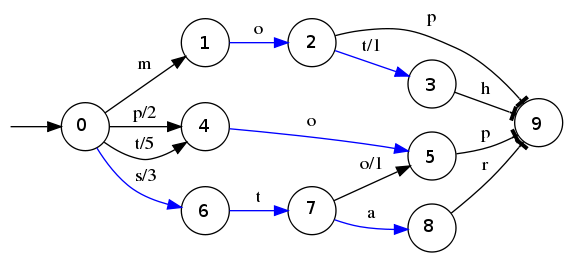
\includegraphics[scale=0.5]{../c_asm/1.png}
    \caption{La FST associée avec le \autoref{tab:fst1} page \pageref{tab:fst1}}
    \label{fig:fst-dico1}
\end{figure}

\begin{table}[ht]
    \centering
    \begin{tabular}{|l||c|c|c|c|c|c|c|c|c|c|c|c|c|c|c|}
        \hline
        N\oe u & 0 & 0 & 0 & 0 & 3 & 3 & 1 & 2 & 4 & 5 & 6 & 5 &\\ \hline
        N\oe u suivant & 1 & 1 & 3 & 4 & 1 & 4 & 2 & 7 & 5 & 6 & 7 & 7 &\\ \hline
        N\oe u final &&&&&&&&&&&&& 7 \\ \hline
        Caractère & P & T & S & M& T & L & O & P & O & T & H & P & \\ \hline
        Poids & 2 & 6 & 3 &  & 2 & & & & & 1 &&& \\ \hline
    \end{tabular}
    \caption{FST utilisée avec le dictionnaire \autoref{tab:dico2}, voir \autoref{fig:fst-dico2} page \pageref{fig:fst-dico2}}
    \label{tab:fst2}
\end{table}

\begin{figure}[!htb]
    \centering
    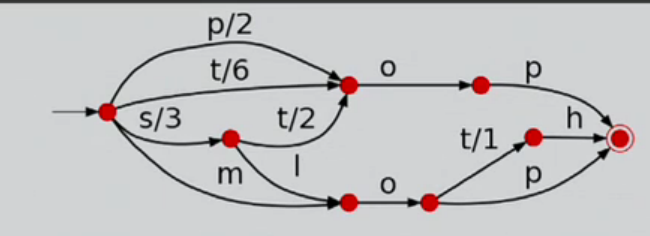
\includegraphics[scale=0.5]{../c_asm/2.png}
    \caption{La FST associée avec le \autoref{tab:fst2} page \pageref{tab:fst2}}
    \label{fig:fst-dico2}
\end{figure}
Les
\clearpage
\subsection{Générer à la volée du code C}
\label{sec:annexe:shell:c}
\subsubsection{Script shell}

\lstinputlisting[style=custombash, caption=Script pour générer un code C à la volée d'une FST,label=lst:bashgen]{../c_asm/gen.sh}

\clearpage
\subsubsection{Code C généré pour la FST définie dans le \autoref{tab:fst1}}

\lstinputlisting[style=customc, caption=Code C généré pour la FST définie dans \autoref{tab:fst1},label=lst:cfst1]{../c_asm/gen_c_fst1.c}

\clearpage
\subsubsection{Code C généré pour la FST définie dans le \autoref{tab:fst2}}

\lstinputlisting[style=customc, caption=Code C généré pour la FST définie dans \autoref{tab:fst2},label=lst:cfst2]{../c_asm/gen_c_fst2.c}


\clearpage
\subsection{Générer à la volée du code assembleur x86}
\label{sec:annexe:shell:asm}
\subsubsection{Script shell}

\lstinputlisting[style=custombash, caption=Script pour générer un code assembleur x86 à la colée d'une FST, label=lst:bashgenasm]{../c_asm/gen_asm.sh}

\clearpage
\subsubsection{Code assembleur x86 généré pour la FST définié dans le \autoref{tab:fst1}}

\lstinputlisting[style=customasm, caption=Code assembleur x86 généré pour la FST définie dans \autoref{tab:fst1}, label=lst:asmfst1]{../c_asm/gen_asm_fst1.asm}

\clearpage
\subsubsection{Code assembleur x86 généré pour la FST définié dans le \autoref{tab:fst2}}

\lstinputlisting[style=customasm, caption=Code assembleur x86 généré pour la FST définie dans \autoref{tab:fst2}, label=lst:asmfst2]{../c_asm/gen_asm_fst2.asm}

\clearpage

\section{Annexe : générer du code java dynamiquement}

\subsection{Dans une seule méthode}

\subsubsection{Avec différents états représentés par des méthodes}


\lstinputlisting[style=customjava, caption=Code Java générant une structure avec des n\oe uds, label=lst:javagen1]{code/FstGeneratorFirstVersion.java}

\clearpage
\subsubsection{Uniquement avec des switch}

\lstinputlisting[style=customjava, caption=Code Java générant une structure switch, label=lst:javagen2]{../java/src/main/java/generator/FstGenerator.java}

\clearpage
\subsection{Dans différentes méthodes}

\lstinputlisting[style=customjava, caption=Code Java générant une structure switch avec fonctions, label=lst:javagen3]{../java/src/main/java/generator/BigFstGenerator.java}

\end{document}
